\chapter{Studie}
\label{kap:Kapitel04}

\section{Simulation}
Die Simulation ist die Grundlage der Evaluation der durchgeführten Studie. Sie soll in erster Linie zeigen, dass die Implementierung des Q-Learning Algorithmus fehlerfrei funktioniert und es für einen Agenten damit möglich ist das Verhalten eines Nutzers zu erlernen. \\
Dazu bedarf es allerdings Testdaten welche das Kaffeetrinkverhalten eines Users repräsentieren. Im \quotes{Simulator} wird es wie folgt umgesetzt.\\
Abstrakt gesehen wird ein virtueller User anhand von Zufallszahlen einer Normalverteilung simuliert.\\
Genauer betrachtet werden die Zeiten, an denen dieser virtuelle User einen Kaffee trinkt, basierend auf der Ziehung von Zahlen aus einer Normalverteilung erzeugt.\\ Dabei wird pro Tag (Montag-Freitag) und in jedem Timeslot (T0-T4) unter Berücksichtigung einer vordefinierten Abweichung und Erwartungswert (siehe \ref{tab:meandevtable}), die Anzahl der getrunkenen Kaffees ermittelt. Für jeden Kaffee wird zufällig eine Uhrzeit gezogen, welche sich in dem Zeitraum des Timeslots befindet. Somit wird ein Trainingsset für den Agenten erstellt, welches das Verhalten einer realen Person in einem Zeitraum von einer Woche abbildet.

\begin{center}
    \captionof{table}{Normalverteilung Tabelle}
    \label{tab:meandevtable}
    \begin{tabular}{| l | l | l |}
    \hline
    Timeslot & Erwartungswert & Abweichung \\ \hline
    0 & 1,0 & 1,0 \\ \hline
    1 & 1,5 & 0,2 \\ \hline
    2 & 1,5 & 0,01 \\ \hline
    3 & 0,2 & 0,5 \\ \hline
    4 & 0,0 & 0,0 \\ \hline
    \end{tabular}
\end{center}


Der Pseudocode des Simulators sieht folgendermaßen aus (vgl. Algorithmus \ref{algo:sim}):

\begin{algorithm}
    \caption{Simulation algorithm}\label{algo:sim}
    \begin{algorithmic}[1]
    \State \emph{weeks} $\gets$ x   \hfill         //x = Anzahl der Episoden
       \For{weeks}
       \State \emph{trainSet} $\gets$ $generateTrainingsSet()$
       \For{$1 \leq day \leq 6$}    \hfill         //Montag-Freitag
       \For{$7 \leq ts < 19$}       \hfill         //Timeslot 0-4
       \State \emph{times} $\gets$ $trainSet[\emph{day}][\emph{ts}]$
       \ForAll {$time \in times$}
       \State $learn(\emph{time})$
       \EndFor
                \EndFor
            \EndFor
       \EndFor
    \end{algorithmic}
    \end{algorithm}

Zuerst wird eine bestimmte Anzahl an Episoden bzw. Wochen festgelegt. In der Simulation waren es 250. Daraufhin wird pro Woche ein Trainingsset mit einem neuen Seed erzeugt, mit welchem der Agent trainiert wird. Durch das Setzen eines neuen Seeds wird vermieden, dass der Agent stets mit dem selben (Wochen) Trainingsset konfrontiert wird. Stattdessen wird mit jeder neuen Episode ein Trainingsset erzeugt, welches komplett neue Uhrzeiten beinhaltet, die jedoch nach der selben Normalverteilung gezogen worden sind.\\
Pro Episode wird zuerst über die Tage (Montag-Freitag), dann über den Zeitraum der Timeslots (7 Uhr - 18 Uhr) und schließlich über die Zeiten an denen der virtuelle User einen Kaffee trinkt iteriert und der Agent letztendlich trainiert.\\

\section{Testphase}
\label{sec:testphase}

Die Dauer der Testphase betrug 3,5 Wochen und umfasste 8 Teilnehmer des Lehrstuhls. Der Versuchsaufbau entsprach dem der Systemarchitektur aus Kapitel \ref{kap:Kapitel03}. \\
Wurde ein Getränk durch einen Mitarbeiter in der App ausgewählt und bestätigt, erfolgte eine Transaktion auf der Blockchain. Jene wurde wiederum vom Learner detektiert, gefiltert und die Daten zur Modellierung des Kaffeetrinkverhaltens verwendet. Zudem wurde jede Prediction und dessen Evaluierung geloggt, sowie in einer Datei abgespeichert. Unter Hilfenahme dieser Log-Datei erfolgte schließlich auch die Auswertung der Ergebnisse.\\\\
Bevor jedoch auf die Evaluierung eingegangen wird, sollen zunächst die Probleme und Hindernisse geschildert werden, die während der Testphase auftraten und die Laufzeit auf lediglich 3,5 Wochen reduzierten.\\
Das Hauptproblem war die veraltete Hardware des Tablets, welche nur noch ein Update auf eine 7 Jahre alte Android Version (4.2.1) zuließ. Mit dieser Version war es nicht möglich, eine direkte Verbindung zum Universitätsnetzwerk per WLan herzustellen, da das benötigte Zertifikat diese Version nicht unterstützt. Eine Verbindung zum Netzwerk ist aber notwendig, um mit der Blockchain zu kommunizieren bzw. eine Transaktion auslösen zu können. \\
Durch einen Workaround (freies WLan + VPN-Client) konnte das Tablet mit dem Universitätsnetzwerk verbunden werden. Trotz alle dem sorgte diese Konstellation für viele unerwartete Verbindungsabbrüche, was dazu führte, dass einige Transaktionsdaten verloren gingen. \\
Um den Verbindungsabbrüchen entgegenzuwirken wurde daraufhin ein Mechanismus implementiert (vgl. \ref{subsec:internalFlow}), welcher zwar zu einer Verbesserung und Erhaltung der Daten beitrug, das Kernproblem allerdings nicht lösen konnte. \\ 
Denn ein Verbindungsabbruch führte oftmals dazu, dass das Blockchain-Modul (Ethereum Library) der App abstürzte und die App manuell geschlossen und neu gestartet werden musste, damit wiederholt eine Verbindung zur Blockchain hergestellt werden konnte. \\
Erst durch den schlussendlichen Setup (Verbindung über einen Hotspot eines Laptop) konnten die Abstürze auf ein Minimum reduziert werden.\\\\
Ein weiteres Hindernis welches während der Testphase auftrat, war das Fehlen (Urlaub) einiger Mitarbeiter über den Zeitraum von 1-2 Wochen hinweg. Dadurch wurden lediglich zwei Datensätze erzeugt, welche als Grundlage für die Evaluation verwendet werden konnten. 

\newpage
\section{Evaluation}

\nlparagraph{Simulation 1}
Bei der ersten Simulation (vgl. Abbildung \ref{img:sim1}) ist eine Konvergenz hin zu einer 100\textit{\%} \quotes{success rate} nach ca. 170 Episoden bzw. Wochen zu erkennen. Dies bedeutet, der Agent hat nach dieser Anzahl an Durchläufen das Kaffeetrinkverhalten des Users in voller Gänze erlernt. \\
Die anfänglichen großen Sprünge, v.a. zwischen den Episoden 5 und 15, sowie 50 und 60, sind charakteristisch für einen Reinforcement Algorithmus. So ist anfänglich die Rate für die Exploration in der Regel sehr hoch, was oftmals zu vielen falschen Predictions führt, da die Aktionen zufällig ausgewählt werden. Mit der Zeit wird diese Rate aber nach und nach verringert und die Sprünge werden weniger. \\
Ein weiteres Merkmal des Graphs ist die logarithmische Trendlinie. Diese ist zum einen auch auf die Reduktion der Exploration zurückzuführen. Zum anderen ist sie dem Lernerfolg des Agenten geschuldet, welcher allerdings erst durch die anfängliche Exploration des Zustandraums ermöglicht wird.


\begin{figure}[th!]
	\centering
	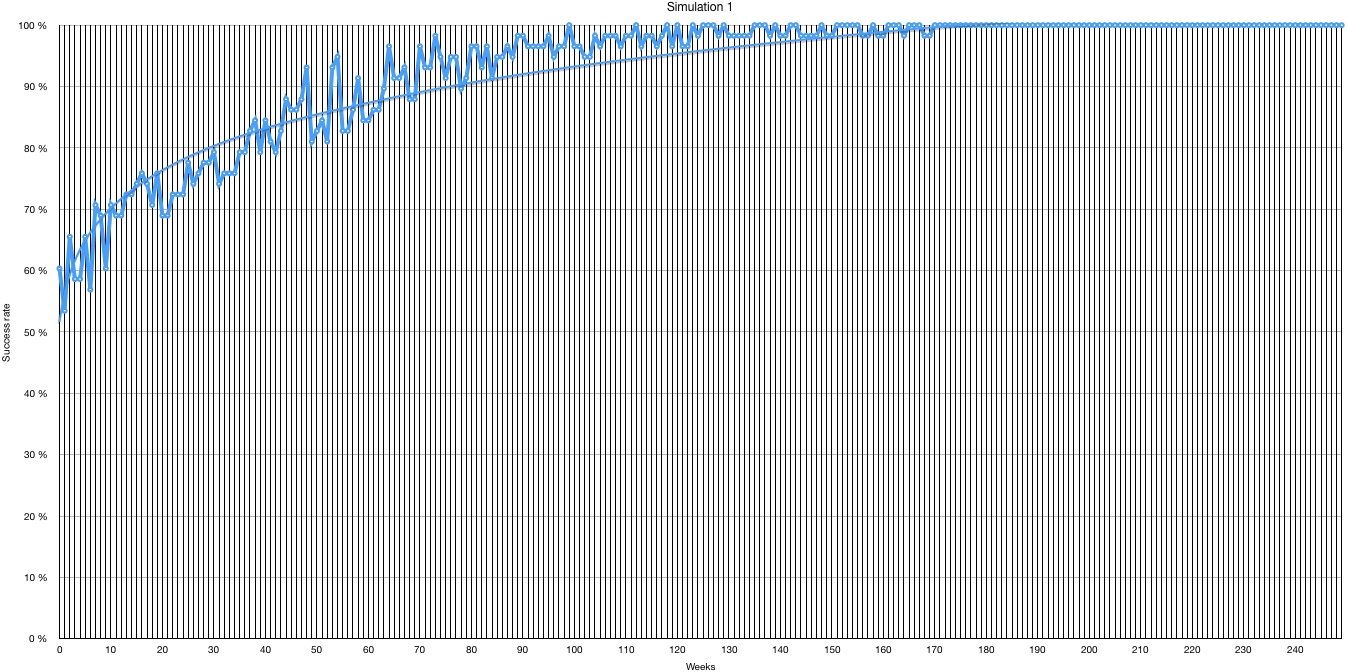
\includegraphics[width=.9\columnwidth]{./Abbildungen/Kapitel_04/sim1.png}
	\caption{Simulation 1: Lernkurve}
	\label{img:sim1}
\end{figure}


\begin{figure}[th!]
	\centering
	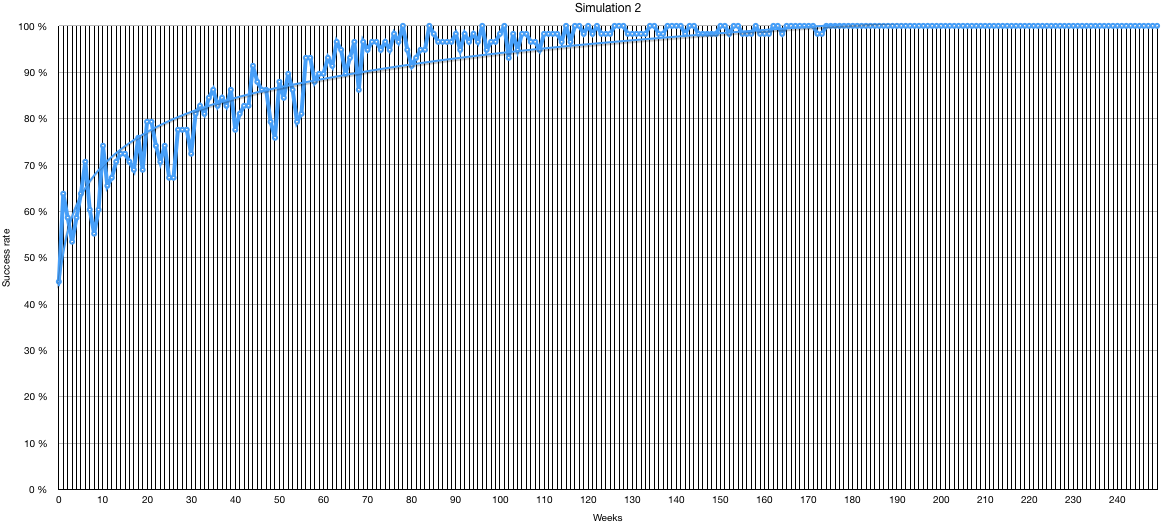
\includegraphics[width=.9\columnwidth]{./Abbildungen/Kapitel_04/sim2.png}
	\caption{Simulation 2: Lernkurve}
	\label{img:sim2}
\end{figure}


\nlparagraph{Simulation 2}
Der Graph der 2. Simulation (vgl. Abbildung \ref{img:sim2}) ist dem der Ersten äußerst ähnlich. So nähert sich dieser dem Optimum auch logarithmisch an und erreicht eine 100\textit{\%} \quotes{success rate} bei ca. 170 Episoden.\\
Aufgrund des sehr hohen Grads der Ähnlichkeit beider Graphen, wird hier auf eine weitere Interpretationen des Verlaufs verzichtet. \\
So sollen lediglich die Ergebnisse der ersten Simulation nochmals untermauert und die einwandfrei Funktionalität der Implementierung des Q-Learning Algorithmus gezeigt werden. 

\nlparagraph{Testphase}
Unter Berücksichtigung der in \ref{sec:testphase} geschilderten Probleme, gilt der Hinweis, dass während der Testphase nur sehr kleine Datensätze für die Evaluation erzeugt wurden. Dadurch erfolgt die Beantwortung der Forschungsfrage nur anhand von abgeleiteten Tendenzen aus den Datensätzen und lässt einen vollständigen Beweis außen vor.  \\
Aus den fünf vorhandenen Datensätzen wurden jeweils zwei zur Auswertung herangezogen, bei denen am häufigsten Feedback durch den User gegeben wurde.\\

\begin{figure}[t!]
    \centering
    \parbox{6cm}{
    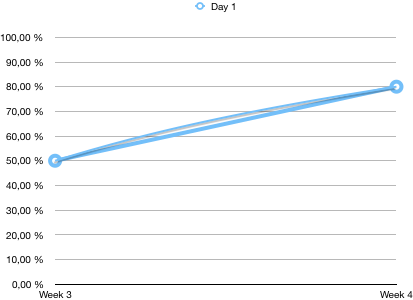
\includegraphics[width=6cm]{./Abbildungen/Kapitel_04/usr1day1.png}
    \caption{User 1: \\Montag}
    \label{img:usr1day1}}
    \qquad
    \begin{minipage}{6cm}
    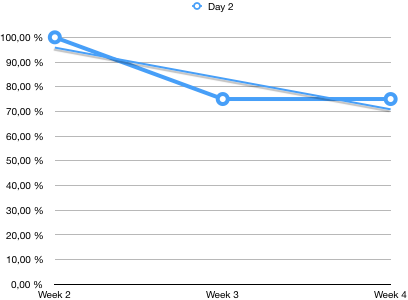
\includegraphics[width=6cm]{./Abbildungen/Kapitel_04/usr1day2.png}
    \caption{User 1: \\Dienstag}
    \label{img:usr1day2}
    \end{minipage}
\end{figure}


\begin{figure}[t!]
    \centering
    \parbox{6cm}{
    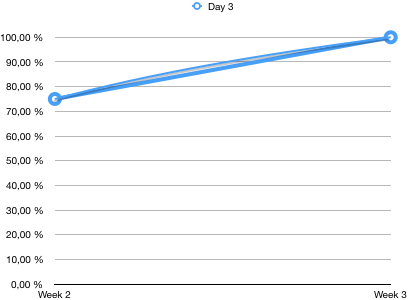
\includegraphics[width=6cm]{./Abbildungen/Kapitel_04/usr1day3.png}
    \caption{User 1: \\Mittwoch}
    \label{img:usr1day3}}
    \qquad
    \begin{minipage}{6cm}
    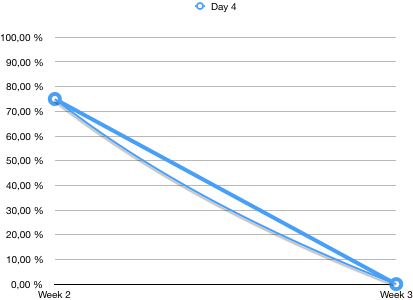
\includegraphics[width=6cm]{./Abbildungen/Kapitel_04/usr1day4.png}
    \caption{User 1: \\Donnerstag}
    \label{img:usr1day4}
    \end{minipage}
\end{figure}

\nlparagraph{User 1}
User 1 wurde erst in der zweiten Woche aktiv, weswegen die Teilnahmedauer nur 2,5 Wochen betrug. 
Betrachtet man den Graphen des Wochenüberlicks (vgl. Abbildung \ref{img:usr1wa}), startet dieser bei einer Erfolgsrate von 75\textit{\%}, fällt in der Woche 3 auf 60\textit{\%} ab und steigt in Woche 4 auf 77,8\textit{\%}. Was daraufhin deutet, dass der Agent aus der Explorationsphase in Woche 3 neues Wissen schöpfen und in Woche 4 anwenden konnte.\\
In Anbetracht der Tagesgraphen, ist im Falle von 3 Tagen (Montag, Mittwoch, Freitag; vgl. \cref{img:usr1day1,img:usr1day3,img:usr1day5}) ein Anstieg der Erfolgsrate um ca. 30\textit{\%} zu erkennen. \\
Der enorme Einbruch an Tag 4 (vgl. Abbildung \ref{img:usr1day4}) von 75\textit{\%} auf 0\textit{\%}, schließt auf ein zur Vorwoche stark verändertes Verhalten des Users. Auch eine Explorationsphase wäre theoretisch denkbar, ist statistisch aber eher unwahrscheinlich.\\
Trotz der Reduktion der Prediction accuracy an Tag 2 (vgl. Abbildung \ref{img:usr1day2}), liegt die Erfolgsrate immer noch bei 70\textit{\%}, was definitiv ein Indiz für den Lernerfolg des Agenten ist. 


\begin{figure}[t!]
    \centering
    \parbox{6cm}{
    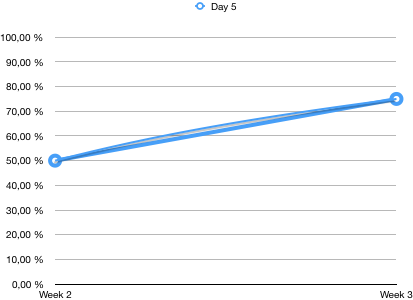
\includegraphics[width=6cm]{./Abbildungen/Kapitel_04/usr1day5.png}
    \caption{User 1: \\Freitag}
    \label{img:usr1day5}}
    \qquad
    \begin{minipage}{6cm}
    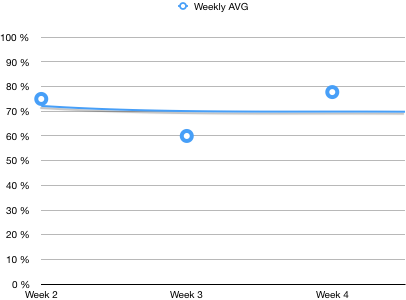
\includegraphics[width=6cm]{./Abbildungen/Kapitel_04/usr1wa.png}
    \caption{User 1: \\Wochenüberlick}
    \label{img:usr1wa}
    \end{minipage}
\end{figure}
    


\clearpage
\newpage

\nlparagraph{User 2}
User 2 war drei Wochen aktiv und startete am 4. Tag der ersten Woche.
Beim Wochenüberblick (vgl. \ref{img:usr2wa}) ist in den Wochen 1-3 zuerst ein Anstieg von 55\textit{\%} auf 68\textit{\%} zu erkennen, welchem anschließend ein Abfall auf eine Erfolgsrate von 44\textit{\%} folgt. \\
Bis auf den dritten Tag ist in allen anderen Fällen (vgl. Abbildung \cref{img:usr2day1,img:usr2day2,img:usr2day4,img:usr2day5})  mindestens einmal ein Anstieg der Erfolgsrate im Vergleich zur Vorwoche zu beobachten. Gerade der Graph des dritten Tages (vgl. Abbildung \ref{img:usr2day3}), bei welchem eine Stagnation über alle 3 Wochen hinweg zu erkennen ist, deutet einerseits auf einen gewissen Lernerfolg hin, zeugt aber auch andererseits von einer fehlenden Exploration des Agenten. \\
Es lässt sich sowohl an den Tagesgraphen, als auch am Wochengraph ein Trend hin zum Lernerfolg des Agenten beobachten. So ist die \quotes{prediction accuracy} in keinem Tag bei 0\textit{\%} und es ist stets ein Anstieg oder zumindest eine Stagnation zu beobachten, was letztendlich auf einen Lernerfolg des Agenten hindeutet.
\\\\
In Anbetracht beider Simulationsergebnisse ist der Lernerfolg bei dieser Problemstellung von logarithmischer Natur. Sowohl der Auswertungsgraph von User 1 (vgl. Abbildung \ref{img:usr1wa}) als auch von User 2 (vgl. Abbildung \ref{img:usr2wa}) teilen diese Charakteristik und zeigen eine Tendenz hin zu einer steigenden Erfolgsrate. Dies würde vorerst die These bestätigen, dass sich Machine Learning und Blockchain verbinden lässt, bzw. das Lernen anhand von Daten einer Blockchain möglich ist. \\
Jedoch muss dies gewissermaßen auch relativiert werden, da die Dauer der Studie sehr kurz war. Die Ergebnisse können eben nur eine Tendenz geben, inwiefern bei einer längeren Dauer der Testphase der Lernerfolg im selben Maße ausfallen würde, wie im Falle der Simulation. \\\\
Schlussendlich bedarf es einer weitaus längeren Studiendauer, um die Forschungsfrage in voller Gänze zu erörtern. 

\begin{figure}[t!]
    \centering
    \parbox{6cm}{
    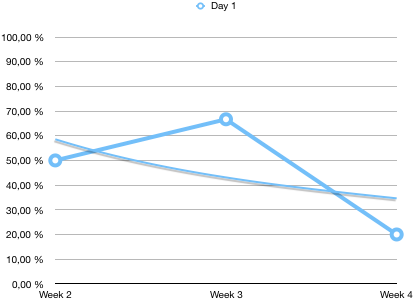
\includegraphics[width=6cm]{./Abbildungen/Kapitel_04/usr2day1.png}
    \caption{User 2: \\Montag}
    \label{img:usr2day1}}
    \qquad
    \begin{minipage}{6cm}
    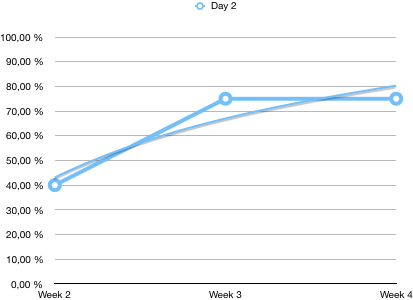
\includegraphics[width=6cm]{./Abbildungen/Kapitel_04/usr2day2.png}
    \caption{User 2: \\Dienstag}
    \label{img:usr2day2}
    \end{minipage}
\end{figure}


\begin{figure}[t!]
    \centering
    \parbox{6cm}{
    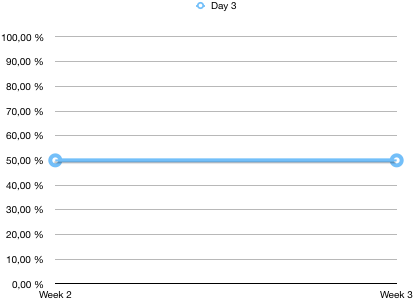
\includegraphics[width=6cm]{./Abbildungen/Kapitel_04/usr2day3.png}
    \caption{User 2: \\Mittwoch}
    \label{img:usr2day3}}
    \qquad
    \begin{minipage}{6cm}
    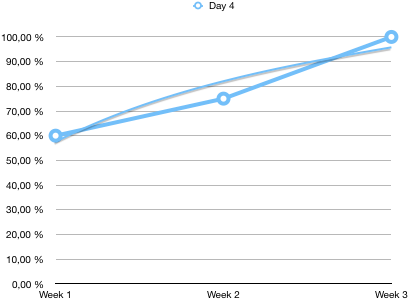
\includegraphics[width=6cm]{./Abbildungen/Kapitel_04/usr2day4.png}
    \caption{User 2: \\Donnerstag}
    \label{img:usr2day4}
    \end{minipage}
\end{figure}

\begin{figure}[t!]
    \centering
    \parbox{6cm}{
    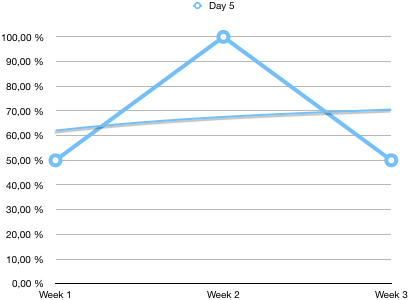
\includegraphics[width=6cm]{./Abbildungen/Kapitel_04/usr2day5.png}
    \caption{User 2: \\Freitag}
    \label{img:usr2day5}}
    \qquad
    \begin{minipage}{6cm}
    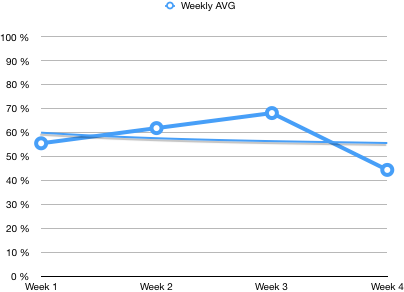
\includegraphics[width=6cm]{./Abbildungen/Kapitel_04/usr2wa.png}
    \caption{User 2: \\Wochenüberlick}
    \label{img:usr2wa}
    \end{minipage}
\end{figure}
